\documentclass[aspectratio=1610,12pt,notheorems]{beamer}

\usepackage[utf8x]{inputenc} \usepackage[russian]{babel}
\usepackage{amsmath,amssymb,amsthm,mathtools}
\usepackage{graphicx,caption,subcaption}
\usepackage{hyperref,natbib}
\usepackage{tikz,xcolor,colortbl,makecell}
\usepackage{algorithm,algpseudocode}
\usepackage{qrcode}

\usetikzlibrary{arrows,backgrounds,patterns,%
	matrix,shapes,fit,calc,shadows,plotmarks,snakes}

\theoremstyle{plain}
\newtheorem{theorem}{Теорема}
\newtheorem{lemma}[theorem]{Лемма}

\theoremstyle{definition}
\newtheorem{definition}{Определение}
\newtheorem{problem}{Задача}

\usetheme[height=0.97cm]{Rochester}
\usecolortheme{dolphin}

\definecolor{hard}{RGB}{145,55,55}
\definecolor{mnsgold}{RGB}{240,235,220}

\setbeamercolor{headline}{bg=hard,fg=mnsgold}
\setbeamercolor*{frametitle}{parent=headline}

\setbeamercolor{structure}{fg=hard}
\setbeamercolor{subsection in head/foot}{bg=white,fg=hard}
\setbeamercolor{section in head/foot}{bg=hard,fg=mnsgold}
\setbeamercolor{block title}{bg=hard,fg=mnsgold}

\setbeamertemplate{navigation symbols}{}

\parskip=2.6mm
\def\ll{\left(} \def\rr{\right)}
\def\lag{\left\langle} \def\rag{\right\rangle}

\definecolor{failpos}{RGB}{230,30,20}
\definecolor{initpos}{RGB}{30,20,220}
\definecolor{turna}{RGB}{100,240,110}
\definecolor{turnb}{RGB}{250,140,110}

\newcommand{\vseper}{\vphantom{$\int_{0_0}^{0^0}$}}

\newcommand{\singlepayoff}[2]{\tikz{
	\draw (0,0) node{\vseper #1}; \draw (0.8,0.8) node{\vseper #2};
}}

\newcommand{\rowdescription}[1]{\tikz{
	\draw (0,0) node{\vseper #1}; \draw (0,0.8) node{\vseper};
}}

\newcommand{\coldescription}[1]{\tikz{
	\draw (0,0) node{\vseper}; \draw (0.8,0) node{\vseper #1};
}}

\newcommand{\myref}[2]{\href{#1}{\texttt{\underline{#2}}}}

\def\mitem{\medskip\item}
\def\ps{\\ [0.65cm]} \linespread{1.16}
\def\fram#1#2{\begin{frame}\frametitle{#1}#2\end{frame}}
\def\usl#1#2{\begin{block}{#1} #2 \end{block} \medskip\pause}
\def\uslnp#1#2{\begin{block}{#1} #2 \end{block} \medskip}
\def\mov#1#2{\begin{scope}[xshift = #1 cm] #2 \end{scope};}

\def\divsby{\mathrel{\rlap{.}\rlap{\raisebox{0.55ex}{.}}\raisebox{1.1ex}{.}}}
\definecolor{starvert}{RGB}{110,175,230}
\newcommand{\vfi}{\varphi}
\newcommand{\litem}{\vspace{0.5cm}\item}

\newcommand{\nkstar}[2]{
	\foreach \i in {1,...,#1} {\draw[thick] (90 + 360 * \i / #1 : 3.5)
		-- (90 + 360 * \i / #1 + 360 * #2 / #1 : 3.5);}
	\foreach \i in {1,...,#1} {\fill[starvert] (90 + 360 * \i / #1 : 3.5) circle[radius=0.16cm];}
}

\title[Introduction to Game Theory]
    {\bfseries Простые, но важные \\ инструменты теории игр}

\author[\ ]
	{Б. А. Золотов,\quad Олимпиада «Математика НОН-СТОП»\\ \vspace{0.3cm}
		{\small Фонд «Время Науки»}}

\institute[\ ]{\ }

\date{\today}

%%%%%%%%%%%%%%
%%%%%%%%%%%%%%

\begin{document}

\frame{\titlepage}

\begin{frame} \begin{center}
	{\Large К чему скриншотить презентацию,\smallskip\\
		когда можно её скачать} \\ [0.9cm]
	{\small Слайды доступны по ссылке: \url{http://bit.ly/spbtym-game-theory}}
\end{center} \end{frame}

\begin{frame} \frametitle{Игры с олимпиад}
	Они же — игры с полной информацией.

\begin{itemize} \itemsep=2.25mm
	\item Множество позиций
	\item Игроки делают ходы по очереди
	\item Игрокам известны все возможные ходы из каждой позиции
	\item На некоторых позициях определяется исход игры, \\
		например — «проигрывает тот, кто не может сделать ход».
\end{itemize}
\end{frame}

\begin{frame} \frametitle{Симметрия ещё глупее}
	Есть две кучи по 100 монеток. Можно вынуть сколько угодно \\
	монеток из одной кучи.
	\medskip \pause

\begin{center} \tikz[scale=1.35]{
\draw (-0.5,0) rectangle ++(-0.7,1.2) (0.5,0) rectangle ++(0.7,1.2);
\filldraw[fill=turnb] (-0.5,1.2) rectangle ++(-0.7,0.85);
\filldraw[fill=turna] (0.5,1.2) rectangle ++(0.7,0.85);
} \end{center}
\end{frame}

\begin{frame} \frametitle{Кто выигрывает при правильной игре?}
	Правильная игра — никто из игроков не знает, какой ход \\
	его соперник сделает следующим. \bigskip
	
	Нет ни игры «в поддавки», ни игры «в худший случай». \\
	Нельзя сводить рассмотрение такой игры к рассмотрению \\
	одного варианта поведения противника.
\end{frame}

\begin{frame} \frametitle{Что такое выигрышная стратегия}
	Это правило, которое описывает ответы данного игрока \\
	на {\it любые} ходы его противника и при {\it любых} \\
	ходах противника приводит к выигрышу. \bigskip
	
	Мы должны уметь отвечать на любой возможный ход — \\
	разумеется, по-разному. Во всех разумных играх стратегия \\
	существует, причём только у одного игрока.
\end{frame}

\begin{frame} \frametitle{Ничья}
	Изредка бывает, что выигрышных стратегий нет, \\
	каждый игрок может не проигрывать. \medskip

\begin{center} \tikz[scale=0.94]{
	\fill[initpos,rotate=90] (1,-0.075) rectangle (1.5,0.075);
	\fill[black,rotate=150] (1,-0.075) rectangle (1.5,0.075);
	\fill[black,rotate=210] (1,-0.075) rectangle (1.5,0.075);
	\fill[black,rotate=270] (1,-0.075) rectangle (1.5,0.075);
	\fill[failpos,rotate=330] (1,-0.075) rectangle (1.5,0.075);
	\fill[black,rotate=30] (1,-0.075) rectangle (1.5,0.075);
} \end{center} \medskip

	Дан циферблат, можно смещать стрелку на 2 или\\
	на 4 деления. Проигрывает тот, кто попадает\\
	в красное деление.
\end{frame}


\begin{frame} \frametitle{Симметрия}
	Двое размещают прямоугольники $6 \times 1$ на доске $100 \times 100$. \medskip \pause

\begin{center} \tikz[scale=0.42]{
	\fill[turnb] (-3,-2) rectangle ++(1,6);
	\fill[turna] (3,2) rectangle ++(-1,-6);
	\foreach \x in {-5,...,5} {
		\draw[gray] (-5.5,\x) -- (5.5,\x) (\x,-5.5) -- (\x,5.5);
	}
	\draw[very thick,gray] (0,-5.5) -- (0,5.5) (-5.5,0) -- (5.5,0);
	\draw[very thick, ->] (-1.5,1.5) to[out=20,in=80] (1.5,-1.5);
} \end{center}\medskip

	А если квадраты $2 \times 2$?
\end{frame}

\begin{frame} \frametitle{Тоже симметрия, но в шахматных фигурах}
	Двое по очереди ходят ладьёй по шахматному полю, причём \\
	ходить можно только вниз или влево. \medskip \pause

\begin{center} \tikz[scale=0.42]{
	\draw (0,0) rectangle (8.5,8.5);
	\fill (2.4,2.4) circle[radius=3mm] (6.1,6.1) circle[radius=3mm];
	\draw[very thick,->,turnb] (6.1,5.5) -- (6.1,2.7);
	\draw[very thick,->,turna] (5.8,2.4) -- (3,2.4);
} \end{center}\medskip

	А если доска не квадратная?
\end{frame}

\begin{frame} \frametitle{Камни из кучи}
\begin{itemize} \itemsep=4mm
	\item Дана куча из $k$ камней. За ход можно вынуть из неё от 1 до 7 камней. Проигрывает тот, кто не может сделать ход.
	\item Дана куча из $k$ камней. За ход можно вынуть из неё от 1 до 7, \\ а также 9 камней. Проигрывает тот, кто не может сделать ход.
\end{itemize} \bigskip \pause

Выигрывает второй при $k$, делящемся на 8, и первый иначе.
\end{frame}


\begin{frame} \frametitle{Выигрышные и проигрышные позиции}
Это метод решения задач на игры, который работает почти всегда, \\
если у каждой позиции есть простое описание. \bigskip

Выигрышная позиция — у игрока, начинающего в ней, есть стратегия. \\
Проигрышная — нет стратегии. \bigskip

Например, «последняя» позиция — проигрышная. Позиции, \\
из которых есть ход в «последнюю», — выигрышные.
\end{frame}

\begin{frame} \frametitle{Теорема о характеризации позиций}
Выигрышные позиции — такие, из которых есть ход \\
хотя бы в одну проигрышную. \bigskip

Проигрышные позиции — такие, ходы из которых \\
только в выигрышные. \bigskip

В соответствии с этим утверждением можно проанализировать \\
все позиции, начиная с конечной.
\end{frame}

\begin{frame} \frametitle{Примеры}
В куче $n$ камней, из неё можно вынуть $a_1$, $a_2$, \ldots, $a_k$ камней. \\
0~камней — проигрышная позиция, остальные расставим. \pause

Двое ходят королём по шахматной доске, можно ходить \\
только вниз, влево или вниз-влево. \pause

\begin{center} \tikz[scale=0.46]{
	\fill[turna] (0,0) rectangle (8,8);
	\foreach \x in {0,2,4,6} {
	    \foreach \y in {0,2,4,6} {
		\fill[turnb] (\x,\y) rectangle ++(1,1);
	    }
	}
	\foreach \x in {0,...,8} {
		\draw[gray] (0,\x) -- (8,\x) (\x,0) -- (\x,8);
	}
} \end{center}
\end{frame}

\begin{frame} \frametitle{Игра Ним}
	Имеется $k$ кучек, в них $N_1$, $N_2$, \ldots, $N_k$ камней. Можно вынуть сколько угодно камней, но только из одной кучи. \medskip

\begin{center} \tikz[scale=1.3]{
	\draw (0,0) rectangle ++(0.6,1.2);
	\draw (1,0) rectangle ++(0.6,1.7);
	\draw (2,0) rectangle ++(0.6,0.9);
	\draw (3,0) rectangle ++(0.6,1.5);
	\draw (4,0) rectangle ++(0.6,1.2);
	\draw (5,0) rectangle ++(0.6,0.8);
}\end{center}
\end{frame}


\begin{frame} \frametitle{Ним-сумма}
	Переведём размеры кучек в двоичную систему и сложим \\
	без переноса разрядов.

	То же самое, что разложить в сумму степеней двойки \\
	и посмотреть, каких из них нечётное число. \medskip

\begin{center}\begin{tabular}{cccc}
2 & 8 & 10 & 11 \\
{\small 10} & {\small 1000} & {\small 1010} & {\small 1011}
\end{tabular}

Ним-сумма — $1011$. \end{center}
\end{frame}

\begin{frame} \frametitle{Свойства ним-суммы} \ \\ [-0.4cm]
	Коммутативна, ассоциативна, $x \oplus x = 0$. \vspace{-0.8cm}
\renewcommand{\sb}{S_{\text{before}}}
\newcommand{\sa}{S_{\text{after}}}

\begin{align*}
&	\sa = \sa \oplus 0 = \sa \oplus \sb \oplus \sb = \\
= &	(x_1 \oplus y_1) \oplus \ldots \oplus (x_k \oplus y_k) \oplus \sb = \\
= & (x_i \oplus y_i) \oplus \sb \\
\end{align*} \vspace{-1.3cm} \pause

$y_i = x_i \oplus (x_i \oplus \sb)$, тогда $x_i \oplus x_i \oplus \sb \oplus \sb = 0$. \pause

\begin{center}\begin{tabular}{cccc}
2 & 8 & 10 & 11 \\
{\small 10} & {\small 1000} & {\small 1010} & {\small 1011} \\
\multicolumn{4}{c}{Ним-сумма — $1011$.} \\ \pause
\phantom{ававав} & \phantom{ававав} & \phantom{ававав} & \phantom{ававав} \\
{\small $1001$} & {\small $11$} & {\small $1$} & {\small $0$} \\
\end{tabular} \end{center}
\end{frame}

\begin{frame} \frametitle{Позиции в игре Ним}
\begin{itemize} \itemsep=5mm
	\item Из любой позиции с ненулевой ним-суммой можно походить \\
	в позицию с нулевой.
	\item При ходе из любой позиции с нулевой ним-суммой — \\
	она становится ненулевой.
	\item Значит, позиции с нулевой ним-суммой — проигрышные, \\
	с ненулевой — выигрышные.
\end{itemize}
\end{frame}


\begin{frame} \frametitle{Ним и другие игры}
	Ним с двумя кучами: выигрышные позиции — когда кучи одинаковы. \\
	Уже было сегодня. \pause

	Шоколадка, одна долька отравлена. Игроки по очереди отламывают и \\
	съедают неотравленную часть. \pause

\begin{center} \tikz[scale=0.44]{
	\fill[turnb] (3,2) rectangle ++(1,1);
	\foreach \x in {0,...,10} {
	   \foreach \y in {0,...,7} {
		\draw[gray] (\x,0) -- (\x,7) (0,\y) -- (10,\y);
	   }
	}
	\draw[thick] (0,5) -- (10,5);
	\foreach \x in {0,2,3,7} {\draw (-1,\x) -- (-0.6,\x);}
	\foreach \x in {0,3,4,10} {\draw (\x,-1) -- (\x,-0.6);}
	\draw[->,thick] (-0.8,3) -- (-0.8,7);
	\draw[->,thick] (-0.8,2) -- (-0.8,0);
	\draw[->,thick] (3,-0.8) -- (0,-0.8);
	\draw[->,thick] (4,-0.8) -- (10,-0.8);
} \end{center}
\end{frame}

\begin{frame} \frametitle{Некооперативные игры}
\begin{center}
\begin{tabular}{|c|c|c|} \hline
	& \coldescription{Split} & \coldescription{Steal} \\ \hline
	\rowdescription{Split} & \singlepayoff{5}{5} & \singlepayoff{0}{10} \\ \hline
	\rowdescription{Steal} & \singlepayoff{10}{0} & \singlepayoff{0}{0} \\ \hline
\end{tabular}\hspace{1.1cm}
\begin{tabular}{|c|c|c|} \hline
	& \coldescription{Cooperate} & \coldescription{Defect} \\ \hline
	\rowdescription{Coop.} & \singlepayoff{3}{3} & \singlepayoff{0}{7} \\ \hline
	\rowdescription{Def.} & \singlepayoff{7}{0} & \singlepayoff{1}{1} \\ \hline
\end{tabular}
\end{center}
\end{frame}

\begin{frame} \frametitle{Некооперативные игры}
\begin{center}
\begin{tabular}{|c|c|c|} \hline
	& \coldescription{Whale} & \coldescription{Fish} \\ \hline
	\rowdescription{Whale} & \singlepayoff{2}{2} & \singlepayoff{0}{1} \\ \hline
	\rowdescription{Fish} & \singlepayoff{1}{0} & \singlepayoff{1}{1} \\ \hline
\end{tabular}\hspace{1.1cm}
\begin{tabular}{|c|c|c|} \hline
	& \coldescription{Swerve} & \coldescription{Straight} \\ \hline
	\rowdescription{Swe.} & \singlepayoff{0}{0} & \singlepayoff{$-1$}{$+1$} \\ \hline
	\rowdescription{Str.} & \singlepayoff{$+1$}{$-1$} & \singlepayoff{$-1000$}{$-1000$} \\ \hline
\end{tabular}
\end{center}
\end{frame}

\begin{frame} \frametitle{Некооперативные игры}
\begin{center}
\begin{tabular}{|c|c|c|} \hline
	& \coldescription{Bach} & \coldescription{Stravinsky} \\ \hline
	\rowdescription{Bch.} & \singlepayoff{2}{1} & \singlepayoff{0}{0} \\ \hline
	\rowdescription{Str.} & \singlepayoff{0}{0} & \singlepayoff{1}{2} \\ \hline
\end{tabular}\hspace{1.1cm}
\begin{tabular}{|c|c|c|} \hline
	& \coldescription{Head} & \coldescription{Tail} \\ \hline
	\rowdescription{Hd.} & \singlepayoff{$+1$}{$-1$} & \singlepayoff{$-1$}{$+1$} \\ \hline
	\rowdescription{Tl.} & \singlepayoff{$-1$}{$+1$} & \singlepayoff{$+1$}{$-1$} \\ \hline
\end{tabular}
\end{center}
\end{frame}

\begin{frame} \frametitle{Эффективность по Парето}
	Нельзя увеличить чей-либо выигрыш без уменьшения выигрыша других.
	
	Соответствует интуитивному представлению о максимальном выигрыше. \pause

\begin{center}
\begin{tabular}{|c|c|c|} \hline
	& \coldescription{Cooperate} & \coldescription{Defect} \\ \hline
	\rowdescription{Coop.} &\cellcolor{turnb} \singlepayoff{3}{3} & \singlepayoff{0}{7} \\ \hline
	\rowdescription{Def.} & \singlepayoff{7}{0} & \singlepayoff{1}{1} \\ \hline
\end{tabular}
\end{center}
\end{frame}

\begin{frame} \frametitle{Равновесие Нэша}
	Действие каждого игрока — наилучшее возможное при известных стратегиях других игроков.
	
	Ни один участник не может увеличить свой выигрыш, если стратегии других игроков неизменны. \vspace{-0.2cm} \pause
	
\begin{center}
\begin{tabular}{|c|c|c|} \hline
	& \coldescription{Cooperate} & \coldescription{Defect} \\ \hline
	\rowdescription{Coop.} & \singlepayoff{3}{3} & \singlepayoff{0}{7} \\ \hline
	\rowdescription{Def.} & \singlepayoff{7}{0} &\cellcolor{turna} \singlepayoff{1}{1} \\ \hline
\end{tabular}
\end{center}
\end{frame}

\begin{frame} \frametitle{Существование равновесия Нэша}
\begin{center}
\begin{tabular}{|c|c|c|} \hline
	& \coldescription{Head} & \coldescription{Tail} \\ \hline
	\rowdescription{Hd.} &
		\singlepayoff{\textcolor{turna}{$+1$}}{$-1$} &
		\singlepayoff{$-1$}{\textcolor{turnb}{$+1$}} \\ \hline
	\rowdescription{Tl.} &
		\singlepayoff{$-1$}{\textcolor{turnb}{$+1$}} &
		\singlepayoff{\textcolor{turna}{$+1$}}{$-1$} \\ \hline
\end{tabular}
\end{center} \medskip \pause

Иногда равновесия Нэша не существует в чистых стратегиях. \\
Но оно всегда есть в {\it смешанных стратегиях.}
\end{frame}

\begin{frame} \frametitle{Пиар «Математики НОН-СТОП»}
\begin{center}
	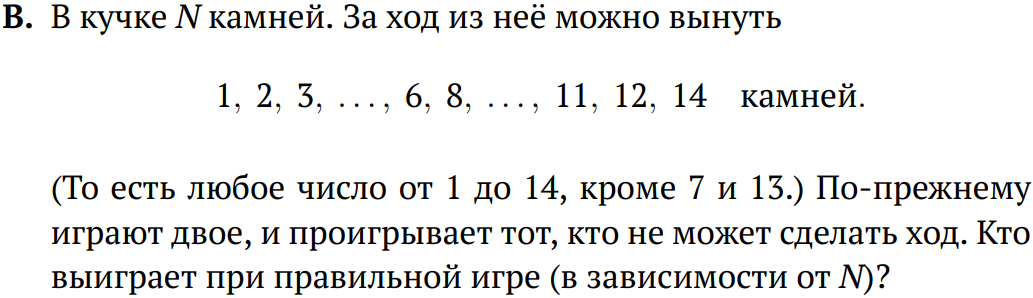
\includegraphics[width=0.7\textwidth]{img/mnsgame} \vspace{1cm}
	
	{\large\tt mathnonstop@timeforscience.ru}
\end{center}
\end{frame}


\def\fitem#1#2{\textcolor{hard}{\small (#1)}~~#2 \medskip \\}

\begin{frame} \frametitle{Заключение}

\textcolor{hard}{\bf Что мы обсудили сегодня}

\fitem{1}{Что такое «правильная игра» и выигрышная стратегия}
\fitem{2}{Игры с симметрией}
\fitem{3}{Дополнение по модулю: от $1$ до $k$ камней из кучи}
\fitem{4}{Как решить любую задачу на игры: В и П позиции}
\fitem{5}{Ним и ним-сумма}
\fitem{6}{Игры — социальные дилеммы \vspace{6mm}}

\hrule
\begin{center}
	{\LARGE Спасибо за внимание!} \smallskip \\
	{\footnotesize \textcolor{hard}{($*$)\quad}
		\url{rs.mathnonstop.ru}
		\phantom{($*$)\quad}}
\end{center} \vspace{2.4mm}
\end{frame}

\end{document}
